\documentclass[12pt]{book}
\usepackage[left=2.5cm,top=3cm,right=2.5cm,bottom=3cm]{geometry}
\usepackage[colorlinks=true,
	        pdftex,
            plainpages=false,
            pdfauthor={Michael Jastram (Ed.)},
            pdftitle={Rodin User's Handbook},
            pdfsubject={Rodin is a platform for Event-B based formal modelling},
            pdfkeywords={Rodin, Event-B},
            pdfproducer={http://handbook.event-b.org},
            pdfcreator={plastex-based tool chain}]{hyperref}
\usepackage{graphicx}
\usepackage{bsymb}
\usepackage{b2latex}
\usepackage{fancyhdr,lastpage,color}
\usepackage{verbatim}
\usepackage{wrapfig}
\usepackage{makeidx}
\usepackage{fix-cm}
\usepackage[utf8]{inputenc}

% Rodin Handbook Version
\newcommand{\versionnr}{2.2}

% Rodin Handbook Version Path. "current" is the newest version of the handbook. This should be changed if we want to build a handbook for another (i.e. older version)
\newcommand{\versionpath}{current}

% Absolute path to handbook
\newcommand{\handbookpath}{http://handbook.cobra.cs.uni-duesseldorf.de}

% We generate an index
\makeindex


% defining a if(plastex) environment
\newif\ifplastex
\plastexfalse

\def\doculist#1#2{
\begin{quote}
\hspace{-10mm}
\textrm{\includegraphics[width=7mm]{#2}} % Hack!  We "mark" the image with textrm so that we can use a different CSS-Style in plastex.
\vspace{-8mm}

#1
\end{quote}
}

\def\tick#1{\doculist{#1}{img/tick_64.png}}
\def\info#1{\doculist{#1}{img/info_64.png}}
\def\warning#1{\doculist{#1}{img/warning_64.png}}
\def\pencil#1{\doculist{#1}{img/pencil_64.png}}

% macro for icons
\def\icon#1{
\includegraphics[]{img/icons/#1}
}

% macro for image versions (pdf version + html version)
% #1 Path to image for pdf version
% #2 Path to image for html version
% #3 Caption
% #4 Label
\def\imagedpi#1#2#3#4#5{
	\ifplastex
		\begin{figure}[!h]
		\begin{center}
			\includegraphics{#3}
			\caption{#4}
			\label{#5}
		\end{center}
		\end{figure}
	\else
		\begin{figure}[!h]
		\begin{center}
			\includegraphics[width=#2]{#1}
			\caption{#4}
			\label{#5}
		\end{center}
		\end{figure}
	\fi
}

% different method to write an ASCII backslash for plastex and normal pdflatex
\ifplastex
  \newcommand{\mybackslash}{\textbackslash}
\else
  % we do not use textbackslash for latex, because it does not use the current font setting
  \newcommand{\mybackslash}{\symbol{`\\}}
\fi

% Path to resources like zip's with machines
% We use a relative path in the html + eclipe version (in order to work offline)
% and an absolute path in the pdf version
\ifplastex
	\newcommand{\filepath}{files/}
\else
	\newcommand{\filepath}{\handbookpath/\versionpath/files/}
\fi

% Use this definition to create a link to the file. The definition takes to arguments. 
% The first argument (1) defines the file name i.e. Celebrity.zip or in case if you saved 
% the file in a subdirectory subdirecotry/Celebrity.zip. The second argument (2) defines 
% the name which should be displayed in the document, i.e. Celebrity Problem Example Download
\def\file#1#2{
\href{\filepath#1}{#2}
}

% We want to mark contributions from other plugins in a special way, by including the plugin's
% icon and by putting the content in a gray box.  We have to approach this differently for
% Latex and for Plastex:
% Latex: We use "shaded" from package "framed"
% Platexte: We use "verse" as the marker and create the shading with the style sheet.
\newcommand{\tmpName}{Dummy}
\ifplastex
\newenvironment{rodin-plugin}[2]
{
\renewcommand{\tmpName}{#2}
  \begin{verse}
\begin{wrapfigure}{l}{}
    \includegraphics{#1}
\end{wrapfigure}
}
{
\newline
\textit{This contribution requires the \textbf{\tmpName} plugin.  The content is maintained by the plugin contributors and may be out of date.}
\end{verse}
}
\else
\usepackage{framed}
\definecolor{shadecolor}{rgb}{0.93,0.93,0.93}
\newenvironment{rodin-plugin}[2]
{
\renewcommand{\tmpName}{#2} % Otherwise we cannot use #2 in the end block - stupid!
\begin{shaded}
\begin{wrapfigure}{l}{10mm}
\vspace{-5mm}
\includegraphics[width=10mm]{#1}
\vspace{-5mm}
\end{wrapfigure}
\noindent
}
{
\vspace{1mm}
\noindent\rule{\textwidth}{.1pt}
\vspace{1mm}
\noindent
{\scriptsize This contribution requires the \textbf{\tmpName} plugin.  The content is maintained by the plugin contributors and may be out of date.}

\end{shaded}
}
\fi

% Marginpars are  cropped - this formats them nicely.
\let\oldmarginpar\marginpar
\renewcommand\marginpar[1]{\-\oldmarginpar[\raggedleft\scriptsize{#1}]
{\raggedright\small{#1}}}
\marginparwidth=2cm

% A command to typeset names of an Event-B section (like variables, invariant, etc)
% consistently.
\newcommand{\eventbsection}[1]{\textsl{#1}}

% A command to typeset consistently the names of proof obligations
\newcommand{\eventbpo}[1]{\textsf{#1}}

% Event-B's finite operator
\newcommand{\bfinite}{\mathrm{finite}}
\newcommand{\bpartition}{\mathrm{partition}}
\newcommand{\bunaryunion}{\mathrm{union}}
\newcommand{\bunaryinter}{\mathrm{inter}}

% Commands for the structure of the reference section

% rrnames is used for the array of operator symbols and description
% at the beginning of a reference section.
% The environment defines an array with three columns:
% 1) The mathematical symbol
% 2) The ASCII representation
% 3) A description of the operator
\newenvironment{rrnames}%
  {\begin{tabular}{l@{\quad---\quad}l@{\quad---\quad}l}}%
    {\end{tabular}}

% The environment rodinrefentry is used for a reference section with several
% entries: Description, Definition, Types, Well-Definedness
% \rrindent is the indention in such an environment
\newlength{\rrindent}
\setlength{\rrindent}{8em}
\newenvironment{rodinrefentry}{%
   \renewcommand\descriptionlabel[1]{\makebox[\rrindent][r]{\textbf{##1}}}
   \setlength{\leftmargini}{\rrindent}
   \begin{description}%
}{%
   \end{description}%
}
\newcommand{\rrdesc}{\item[Description]}
\newcommand{\rrdef}{\item[Definition]}
\newcommand{\rrtypes}{\item[Types]}
%\newcommand{\rrwd}{\item[Well-Definedness]}
\newcommand{\rrwd}{\item[WD]}
\newcommand{\rrfis}{\item[Feasibility]}
\newcommand{\rrex}{\item[Example]}

\newcommand{\actfis}{\mathcal{F}}

% operators (L and D) for well-definendness
\newcommand{\wdl}{\mathcal{L}}
\newcommand{\wdd}{\mathcal{D}}

% a placeholder symbol for operators
\newcommand{\opelipse}{\mathbin{\Box}}

\newcommand{\podef}[4]{%
  \begin{center}
    \setlength{\parindent}{2em}\vspace{0.2em}
    \begin{tabular}{rp{0.5\textwidth}}
      \hline
      & \textbf{#1} \\
      Name       & #2 \\
      Goal       & #3 \\
      Hypotheses & #4 \\
      \hline
    \end{tabular}
  \end{center}
}

% a second approach to proof obligations
\newcommand{\pode}[3]{%
  \begin{center}
    \setlength{\parindent}{2em}\vspace{0.2em}
    \begin{tabular}{rp{0.6\textwidth}}
      \hline
      & \textbf{#1} \\
      Name       & #2 \\
      Goal       & #3 \\
      \hline
    \end{tabular}
  \end{center}
}

%%% Local Variables: 
%%% mode: latex
%%% TeX-master: "rodin-doc"
%%% End: 



\title{Rodin User's Handbook v.\versionnr}
\author{
Work in Progress\\
Handbook $ $Rev$ $ \\
\\
\href{mailto:rodin-handbook@formalmind.com}{rodin-handbook@formalmind.com}\\
\href{http://handbook.event-b.org}{handbook.event-b.org}
}

\begin{document}        

\ifplastex
\maketitle
\begin{center}

\includegraphics{img/rodin_miikka_skaffari_small.jpg}
\end{center}
\else
\begin{titlepage}
\AddToShipoutPicture*{\BackgroundPic}
\vspace*{14.5cm}
{\fontsize{70}{85}\selectfont \bfseries Rodin}

\vspace*{0.2cm}
{\fontsize{24.5}{30}\selectfont \bfseries User's Handbook}

\vspace*{1cm}
{\fontsize{16}{19}\selectfont \textbf{\textsf{Covers Rodin v.\versionnr}}}

\vspace*{1cm}
{\fontsize{16}{19}\selectfont \textsf{Michael Jastram (Ed.)}}

\vspace*{0.2cm}
{\fontsize{16}{19}\selectfont \textsf{Foreword by Prof. Michael Butler}}

\vspace*{1cm}

\includegraphics[width=12mm]{img/deploy-logo.png}

\vspace*{-8.4mm}
\hspace*{12mm}
{ \fontsize{11}{15}\selectfont \textsf{This work is sponsored by the Deploy Project}}

\vspace*{-22mm}

\end{titlepage}
\phantomsection
\addcontentsline{toc}{chapter}{Contents}
\tableofcontents
\fi

\chapter*{Preface}
\addcontentsline{toc}{chapter}{Preface}
\label{preface}

Nobody likes to write documentation, yet everybody agrees that documentation is crucially important.  For a tool platform as complex as Rodin, documentation is necessary if it is supposed to succeed in reaching a wider audience.

The executive team of the DEPLOY project recognized this. In a meeting at ETH in 2010, the team established, amongst other things, that ``it is clear that the current documentation would not support, say, an engineer in an automotive company to start using the tools without significant support''.  It then commissioned the creation of better Rodin documentation.  This handbook is the result of this effort.

Rather than reinventing the wheel, we took all the existing documentation into account, restructured it, extended it where necessary, created plenty of cross-references, and put the resulting document through an editorial process to ensure readability.

A word of warning and encouragement: Don't expect to be an expert in Event-B modelling after reading this handbook.  Its aim is to provide support while getting acquainted with the tool platform. It provides the basics of modelling and can also be used as a companion guide for experts.  Beginners can work their way through the tutorial, which starts with installation and ends with moderately difficult proofs.  Additional support is available in the form of an FAQ and a comprehensive index.  Advanced users can refer to the comprehensive reference section, where they can quickly find essential information regarding the different formalisms.

Whenever the handbook requires former knowledge, it provides links and hints about where to get it.  Whenever it stops, it provides references for further reading.  In particular, it provides plenty of references to the Rodin Wiki, and provides information on how to get in touch with the Rodin community.  We are confident that this handbook will achieve its mission to get new users acquainted with Rodin without frustration and hopefully some with fun.

\begin{flushright}
  Michael Jastram, Düsseldorf, 2012
\end{flushright}

\chapter*{Foreword}
\addcontentsline{toc}{chapter}{Foreword}
\label{foreword}
The Rodin tool supports the application of the Event-B formal method.  It provides core functionality for syntactic analysis and proof-based verification of Event-B models. Rodin also provides extension points for a range of additional plug-ins that enrich the core functionality through support for features such as model checking, model animation, graphical front ends, additional proof capabilities and code generation.While the B Method, developed by Jean-Raymond Abrial in the early 1990s, is focused on supporting formal development of \textit{software}, Event-B broadens the perspective to cover \textit{systems}; instead of just modelling software components, Event-B is intended for modelling and reasoning about systems that may consist of physical components, electronics and software.  An essential difference between Event-B and the B Method is that Event-B admits a richer notion of refinement in which new observables may be introduced in refinement steps; this means that complex interactions between subcomponents may be abstracted from in early stage modelling and then introduced through refinement in incremental stages.  

At around the same time that Jean-Raymond was developing the concepts in Event-B, I was involved in an initiative with the University of Newcastle (Alexander Romanovsky, Cliff Jones), {\AA}bo Akademi  (Kaisa Sere, Elena Troubitsyna) and Jean-Raymond to put together an EU proposal on formal methods for dependable systems.  That became the RODIN project (2004 to 2007) and a key part of the project was the development of an open source extensible toolset to support refinement-based formal development.  Many of Jean-Raymond’s ideas on Event-B were worked into the requirements for the tool and the development of the core tool platform was led by Jean-Raymond and Laurent Voisin (both then at ETH Zurich). Thorough analysis was undertaken to determine that Eclipse was the right platform on which to build an open toolset.  The ease with which the core may be extended with plug-ins from a range of teams to provide seamless functionality indicates this was a good decision. The tools developed in the RODIN project took on the name of the project and, since it had a certain cachet, it was decided to retain the Rodin name for the tool after the project ended.

The RODIN Project was followed by the DEPLOY Project which addressed further development of the Rodin core and associated plug-ins in parallel with industrial-scale deployment of the Rodin tools.  Exposing the tools to serious industrial users in DEPLOY drove the developers to implement significant improvements in performance, usability and stability of Rodin and key plug-ins such as ProB, the Theory plug-in, Camille and UML-B.  Of course, as well as demanding improvements to the tool, the industrial users demanded documentation on the tool, which led to this handbook.  Michael Jastram and the team at D\"{u}sseldorf have done an excellent job in pulling together, extending and improving various sources of documentation on the Rodin tool.  Like the Rodin tools, it will serve as a valuable resource that will continue to evolve beyond the DEPLOY project.

\begin{flushright}Michael Buttler, Southampton, 2012\end{flushright}


\chapter{Introduction}

This handbook provides documentation for users of the Rodin toolset, which provides tools for working with Event-B models.

Event-B is a formal method for system-level modelling and analysis. Key features of Event-B are the use of set theory as a modelling notation, the use of refinement to represent systems at different abstraction levels and the use of mathematical proof to verify consistency between refinement levels.

The Rodin Platform is an Eclipse-based IDE for Event-B that provides effective support for refinement and mathematical proof. The platform is open source, contributes to the Eclipse framework and is further extensible with plugins. 

This handbook covers the use of the core platform.  Documentation for developers and regarding extensions can be found in the Rodin wiki (\ref{rodin_wiki}).

What you see here is a working draft of the documentation.  We are grateful for any feedback that you may have (\ref{feedback}).

\section{Overview}

This handbook consists of five parts:

\begin{description}
	\item[Introduction] You are reading the introduction right now.  Its purpose is to help you orient yourself and to find information quickly.
	\item[Tutorial] If you are completely new to Rodin, the tutorial is a good way to get up to speed quickly.  It guides you through the installation and usage of the tool and gives you an overview of the Event-B modelling notation.
	\item[Reference] The reference section provides comprehensive documentation of Rodin and its components.
	\item[Frequently Asked Questions] Common issues are listed by category in the FAQ.
	\item[Index] We included an index particularly for the print version of the handbook, but it may be useful in the electronic versions as well.  
\end{description}

\subsection{Formats of this Handbook}
\label{handbook_formats}

The handbook comes in various formats:

\begin{description}
	\item[Eclipse Help] The Rodin Handbook is shipped with Rodin and can be accessed through the help system.  The handbook will be updated with the standard Rodin update mechanism.
	\item[Online Help] You can access the handbook online at \url{http://handbook.event-b.org}.
	\item[PDF Help] Both online versions also include a link to the PDF version of the handbook.
\end{description}

\subsection{Rodin Wiki}
\label{rodin_wiki}

This handbook is complemented by the Rodin wiki (\url{http://wiki.event-b.org/}).  Sometimes, the handbook will refer to the wiki for more information.  Also, plugin and developer information is usually located in the wiki.

\subsection{Feedback}
\label{feedback}

All online versions of the handbook contain a button or link for feedback.  Work on the handbook will continue until March 2012, so your feedback will be read and will help to improve this handbook.

You can also submit feedback via email to \texttt{rodin-hand\-book@formal\-mind.com}.

\section{Further Reading}
\label{literature}

In this section, we present a selected list of reading materials that provide information that is not covered in this handbook.

\subsection{Modeling in Event-B: System and Software Engineering, J.-R. Abrial (2010)}
\label{abrial_2010}

This book represents the ultimate authority on Event-B, written by its creator.  The example from Section~\ref{tut_location_access_controller} is based on an example from the book.

From the editor: ``A practical text suitable for an introductory or advanced course in formal methods, this book presents a mathematical approach to modelling and designing systems using an extension of the B formal method: Event-B. Based on the idea of refinement, the author's systematic approach allows the user to construct models gradually and to facilitate a systematic reasoning method by means of proofs. Readers will learn how to build models of programs and, more generally, discrete systems, but this is all done with practice in mind. The numerous examples provided arise from various sources of computer system developments, including sequential programs, concurrent programs and electronic circuits. The book also contains a large number of exercises and projects ranging in difficulty. Each of the examples included in the book has been proved using the Rodin Platform tool set, which is available free for download at www.event-b.org.''

\subsection{Rodin: An Open Toolset for Modelling and Reasoning in Event-B (2009)}
\label{abrialBHHMV_2009}

This article discusses the design principles of the Rodin platform and the Event-B language and 
explains the motivation behind it.

The abstract states: ``[\ldots] we present the Rodin modelling tool that seamlessly integrates modelling and proving. 
 We outline how the Event-B language was designed to facilitate proof and how the tool has been designed to support changes to 
 models while minimising the impact of changes on existing proofs. 
 We outline the important features of the prover architecture and explain how well-definedness is treated. [\ldots]''

The authors J.-R.~Abrial, M.~Butler, S.~Hallerstede, T.~S.~Hoang, F.~Mehta and L.~Voisin have published the article in the journal Software Tools and Technology Transfer (STTT).

\section{Conventions}
\label{conventions}

We use the following conventions in this manual:

\tick{Checklists and milestones are designated with a tick. Here we summarize what we want to learn or should have learned so far.}
\info{Useful information and tricks are designated by the information sign.}
\warning{Potential problems and warnings are designated by a warning sign.}
\pencil{Examples and Code are designated by a pencil.}

We use \texttt{typewriter} font for file names and directories.

We use \textsf{sans serif font} for GUI elements like menus and buttons.  Menu actions are depicted by a chain of elements, separated by ``$\rangle$'', e.g. \textsf{File $\rangle$ New $\rangle$ Event-B Component}.

\section{Acknowledgements}
\label{sec:acknowledgements}

The content of this handbook has been growing since the formation of the European Union IST Project RODIN in 2004.  Giving credit to every contributor is almost impossible and attempting to do so would almost certainly omit some people, which would contradict the spirit of this work.  It should be sufficient to say that we extend our gratitude to all contributors to the Rodin Wiki (\ref{rodin_wiki}). In particular, we would like to thank Systerel\footnote{\url{http://www.systerel.fr}} for their significant contributions to the handbook as they have been the main driver behind the tool and its documentation.

We would also like to thank Cliff Jones, who never gave up the quest to improve the Rodin documentation, and Ken Robinson, who contributed the \file{EventB-Summary.pdf}{Event-B Cheat Sheet}.

We are grateful to the editorial team that made this book possible in the first place, consisting of Daniel Plagge, Lukas Ladenberger and Joy Clark.  We also thank Prof. Michael Leuschel, department head of the institute of software technology and programming languages at the University of Düsseldorf, who supported us in pursuing this project.

The icons that you find throughout this handbook were created by Pixel-Mixer\footnote{\url{http://pixel-mixer.com/}}, who provides them for free.  Thanks!

The cover picture was taken by \href{http://www.skaffari.fi/}{Miikka Skaffari}, who made it available via the Creative Commons by-nc license, depicting a sculpture by Rodin.  Thanks!

\section{DEPLOY}
\label{deploy}

This work has been sponsored by the DEPLOY project\footnote{\url{http://www.deploy-project.eu/}}.  DEPLOY is a European Commission Information and Communication Technologies FP7 project.

The overall aim of the EC Information and Communication Technologies FP7 DEPLOY Project is to make major advances in engineering methods for dependable systems through the deployment of formal engineering methods. Formal engineering methods enable greater mastery of complexity than found in traditional software engineering processes. It is the central role played by mechanically-analysed formal models throughout the system development flow that enables mastery of complexity.

As well as leading to big improvements in system dependability, greater mastery of complexity also leads to greater productivity by reducing the expensive test-debug-rework cycle and by facilitating increased reuse of software.

The goal of the project is to achieve and evaluate industrial take-up of DEPLOY's methods and tools (which started with DEPLOY's industrial partners) as well as to perform further research on methods and tools that is considered necessary.

\section{Creative Commons Legal Code}
\label{sec:cc}        

The work presented here is the result of an collaborative effort
that took many years.  To ensure that access to this work stays free
and to avoid any legal ambiguities, we decided to formally lincense
it under the Creative Commons Share-Alike License.

This work is licensed under the Creative Commons Attribution-ShareAlike 3.0 Unported License. To view a copy of this license, visit \url{http://creativecommons.org/licenses/by-sa/3.0/} or send a letter to Creative Commons, 444 Castro Street, Suite 900, Mountain View, California, 94041, USA.



% \section{Style Guide}

\info{For now, we will manage the style guide as \LaTeX~together with the rest of the documentation.  We may take it out upon publication.}

\subsubsection{General Stylistic Guidelines}

\begin{itemize}
	\item The Conventions (\ref{conventions}) are part of the style guide.

	\item Use the ``we'' form.

	\item We use British English.

	\item When refering to the different views in Rodin, the word ``view'' should be written in lowercase, e.g., the Rodin Problems view.
\end{itemize}

\subsubsection{Files}

Files should be saved in the \texttt{files} subdirectory. You can also create a subdirectory. Then, use the definition 

\begin{verbatim} \file{1}{2} \end{verbatim} 

to create a link to the file. The definition takes to arguments. The first argument (1) defines the file name i.e. \texttt{Celebrity.zip} or in case if you saved the file in a subdirectory \texttt{subdirecotry/Celebrity.zip}. The second argument (2) defines the name which should be displayed in the document, i.e. ``Celebrity Problem Example Download''.

\warning{Please note, that you only enter the file name without a path before (expected subdirectories). The build script assigns automatically the correct path to the file on the server.}

Here is an example using the definition: \file{Celebrity.zip}{Celebrity Problem Example Download}.

\subsubsection{Avoiding Redundancy}

We will reduce (or avoid) redundancy through heavy linking, following these guidelines:

\begin{itemize}
	\item If in doubt, provide the bulk of the information in the Reference section.  For instance, the FAQ entry ``What is Event-B?''  Should simply refer to the Event-B entry in the Reference section.
	\item Web Links should not appear multiple times
	\item Realize web links as footnotes in the Tutorial and FAQ.
	\item Realize web links in a ``See also'' Section in the Reference.
\end{itemize}

\subsubsection{Sections}

\begin{itemize}
	\item If referring to a specific chapter or section, use uppercase to denote this, e.g. ``in Chapter~3''.
	\item We also refer to subsections as Section, e.g. ``see Section~2.5''
	\item We have a small number of well-defined chapters which are the top level structuring element.
	\item Sections and subsections are numbered.  In the HTML-Versions, they are broken into subpages.
    \item Subsubsections do not receive numbers and are not broken into subpages in the HTML.  Keep this in mind regarding both the reading flow and page sizes.
	\item Avoid linking (ref) to subsubsections, as they don't have a number.  Latex will instead provide a link to the next higher element.  This works, but it could create confusion.
	\item Generally, we should avoid gaps in the hierarchy (i.e. having a subsubsection in a section without a subsection in between).\footnote{Coincidentally, this style guide violates this rule. Reason: We want the style guide not broken into subpages, but the proper hierarchy is a section.}
	\item Section labels should be all in lower case. Use ``\_'' for blanks.
	\item We use the prefix ``\texttt{int\_}'' for introduction section labels, ``\texttt{tut\_}'' for tutorial section labels following the section number (i.e. \texttt{tut\_01}) and ``\texttt{faq\_}'' for faq section labels following a short version of the title (i.e. \texttt{faq\_diff\_eventb\_b}). Reference section labels have no prefix.
\end{itemize}

\subsubsection{Images}
\begin{itemize}
	\item Images must be no more than 700 pixels in width (for HTML version)  This is fairly easy for bitmaps (screenshot), pay attention to this regarding how plasTeX converts vector images. (see Latex section below on how to include images)

    \item Screenshots should look neat and consistent.  Horizontal real estate will always be an issue, so please resize the windows before taking the screenshot to keep things readable at 700 pixel width.  (see Latex section below on how to include images)

	\item Images should always have a caption and a label. Please use for the label the same conventions like for the section labels. However, use the prefix ``\texttt{fig\_}''. Example: ``\texttt{fig\_tut\_03\_traffic\_light}''. For referencing do not use references like "As shown bellow" or "Like in the following image:". Use always a format like:

\begin{verbatim}"... as shown in figure \ref{fig_tut_03_traffic_light}."\end{verbatim}

	\item We use icons from Pixel-Mixer, which are free as long as credit is given: \url{http://www.softicons.com/free-icons/toolbar-icons/basic-icons-by-pixelmixer}

  \item We include Window decoration only when it is really necessary.  If we discuss only some views, we crop the rest away.  Please crop neatly, following edges. Even if you need a screenshot with window decoration, you should always use the same Window decoration (i.e. linux ubuntu default decoration style). If you need such a screenshot, please contact Lukas.

  \item Image file names should be all in lower case and not include umlaute or special characters. Use ``\_'' for blanks.

  \item Image files should keep the following rules:
	
\begin{itemize}
		\item Tutorial images should be saved in the sub folder \texttt{img/tutorial} with the prefix ``\texttt{tut\_}'' following the section number. For instance, \texttt{tut\_01\_image1.png}.

		\item FAQ images should be saved in the sub folder \texttt{img/faq} with the prefix ``\texttt{faq\_}''. For instance, \texttt{faq\_image1.png}.

	\end{itemize} 
	\end{itemize} 

\subsubsection{\LaTeX{} Styling}

\begin{itemize}
	\item Try to avoid fancy \LaTeX formatting, as PlasTeX (used for generating HTML) is temperamental.  Especially macros don't always work, and sometimes the result is just ugly.
	\item We have the option to use different files for PDF and HTML generation, but we would generally prefer not to do this.  Look at \texttt{bsymb.sty} and \texttt{plastex-bsymb.sty} as an example. \textbf{NOTE:} We don't do this any more for any style files.
	\item Every section should have a label, reflecting the section name, all lowercase, spaces replaced with underscores (\_).
	\item Don't create subdirectories in the \texttt{latex} folder, as the scripts cannot always deal with them.
	\item Put images in the \texttt{img} folder.  Feel free to create additional directory structures underneath.
	\item Files other than images (e.g. Event-B projects) TODO - we have to figure out whether to keep them in svn (then they won't be accessible from PDFs) or on the Wiki (then they won't be accessible offline).
	\item Don't use hyperlinks for cross-references, but linked section numbers (generated with \texttt{\\ref{}}.  This is necessary for the print documentation to be useful.
	\item When including images in Latex, do not provide a width!  Instead, try to embed the print size in the image itself.  For instance, PNGs allow you to set the print size (in mm).  This way we can be sure that the images are rendered as HTML without distortion.
\end{itemize}

\subsubsection{Contributions from Plugin Developers}
\begin{rodin-plugin}{img/prob.png}{ProB}
We want to encourage Plugin developers to contribute to the Handbook, but we have to make it clear that we cannot maintain that documentation.  Therefore, it has to be clearly marked.  We use a custom environment for that purpose that
\begin{itemize}
	\item Provides the Plugin's icon
	\item Adds a disclaimer to the end of the custom documentation
	\item Puts the content into a gray box (like this one).
\end{itemize}

\end{rodin-plugin}





\chapter{Tutorial}
\label{tutorial}

This tutorial should provide the user with a tour through the most important functionalities of Rodin, so that he gets a understanding of how the program works.

The tutorial doesn't contain all the knowledge that you require.  Instead, it touches upon every concept - from installation to set theory to modeling and refinement - and helps you to find gaps in your knowledge.

Before we build a first model, we will cover some basic math.

\section{Tutorial Proposal (WP1-4)}

These are the chapters of the tutorial.  Average time available to write each chapter: 5 hours.  This is not much time.  Therefore, make sure that the skeleton exists before filling in details.
This is particularly true for screenshots: By all means indicate where screenshots should be, but don't waste time on them until the end.

\begin{description}
	\item[Background before getting started] We give a brief description of what Event-B is and what it is being used for; what kind of background knowledge we expect.
	\item[Installation] We guide the user through downloading, installing and starting Rodin and point out platform differences.  We install the provers.  We name the visible views and describe what they are doing.
	\item[A Machine, and nothing else] We introduce a first machine, a traffic light with booleans for signals. 
      We introduce guards, resulting in the proof obligations to be discharged automatically.
      We explain how proof labels are read, without changing to the proof perspective.
	\item[Mathematical notation] At this point we quickly go through the most important aspects of predicate calculus and provide pointers to the reference and to external literature.  We cover everything used by the traffic light system; we introduce all data types; We introduce sets and relations, but not in depth.  Difference between predicates and expressions; for instance, understand the difference between TRUE and $\top$.  
	\item[Introducing Contexts] We introduce Contexts to apply the theoretical concepts that were introduced in the previous section.  We use the Agatha-Puzzle to step by step introduce more and more complex elements.We point out partitions as a typical pitfall (also add to FAQ).  We will cover Theorems. Well-Definedness is mentioned, but not part of the Agatha-Puzzle.
	\item[Event-B Concepts] This is another theoretical section that provides more background about the previous examples.  For instance, we analyze the anatomy of a machine, introduce all elements that a machine or context may have. We point to literature about the theory, but won't go into the details of the  calculus.  We describe the sees and refines concepts, which will be applied in the next section.  We will briefly mention concepts like data refinement and witnesses, but leave the details to the literature.

	\item[Expanding the Traffic Light System]  We apply what we learned in the previous section by introducing a context with traffic light colors, and a refinement to integrate them.  We will introduce another refinement for the push buttons.

We may structure this and the previous section differently as we develop the tutorial to ensure readability.  But we won't change the content.

	\item[Proving] Hopefully, so far all proof obligations were discharged automatically.  Now we switch for the first time to the proving perspective and explore it.
      We change the auto prover configuration, invalidate proofs and show, that with the new configuration they don't discharge any more.

Here we will solicit feedback from the community to find good examples.


      We prove a simple proof by hand.  We describe the provers available.
	\item[Tricky Proving] We start with a new example that contains a difficult proof.  We walk the user through discharging the proof with plenty of screen shots.
	\item[Complete Abrial Example] We pick an interesting example from the Abrial book, if we get permission.  We could also take one of the Rodin Wiki Tutorial examples (e.g. Location Access Controller).
	\item[Outlook] This concludes the tutorial, but we will provide many pointers to the user.  In particular, we will point to the literature from the Deploy project, the Wiki and to plugins that solve specific problems.
\end{description}

\section{The First Machine: A Traffic Light Controller}
\label{tut_first_machine}

% a first machine, e.g. a traffic light with booleans for signals.  We introduce guards, resulting in the proof obligations to be discharged automatically. We explain how proof lables are read, without changing to the proof perspective.

\tick{\textbf{Goals:} The objective of this section is to get acquainted with the modeling environment. We will create a very simple model consisting of just one file to develop a feeling for Rodin and Event-B.}

In this tutorial, we will create a model of a traffic light controller.  We will use this example repeatedly in subsequent sections.  Figure \ref{fig_tut_03_traffic_light} depicts what we are trying to achieve.

\begin{figure}[!ht]
\begin{center}
	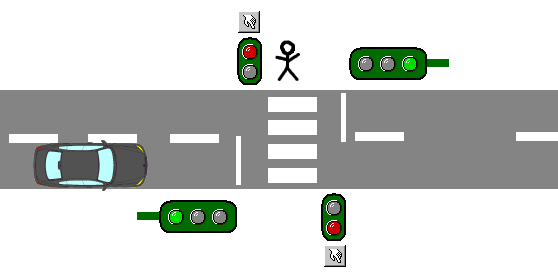
\includegraphics[]{img/tutorial/tut_03_trafficlight.png}
	\caption{The traffic light controller}
	\label{fig_tut_03_traffic_light}
\end{center}
\end{figure}

In this section, we will implement a simplified controller with the following characteristics:
\begin{itemize}
	\item We will model the signals with boolean values to indicate ``stop'' (false) and ``go'' (true).  We do not model colors (yet) because
      we think we should first specify our goal (regulating the traffic) and later we should add implementation details (the traffic light's colors).
	\item Too keep the initial model simple, we will not include the push button yet. We will add it later.
\end{itemize}

\subsection{Excursus: The specification process}
\label{tut_excursus_the_sepcification_process}

While this handbook is concerned with use of the Rodin tool, it's important to understand the specification process as well.  Especially for beginners it can be daunting and unclear where to start with the model, what kind of data structures and abstractions to use, and so on.

We cover a few examples in this chapter that implicitly answer these questions, but there is no explicit set of instructions.  For example, we will first model the traffic lights as booleans, and later refine them into actual colors.  But how did we come up with this refinement strategy?  Likewise, we decided to add the push buttons at a later refinement.  In retrospect this may seem useful, but it leaves open the question on how we arrived at this structure in the first place.

Abrial has something to say about this in his book\footnote{\url{http://www.amazon.com/Modeling-Event-B-System-Software-Engineering/dp/0521895561}}, for which some chapters are available in the Rodin Wiki.

\subsection{Project Setup}
\label{tut_project_setup}

Models typically consist of multiple files that are managed in a project.  Create a new Event-B Project \textsf{File $\rangle$ New $\rangle$ Event-B Project}.  Give the project the name \texttt{tutorial-03} as shown in Figure \ref{fig_tut_03_new_project_wizard}.

\begin{figure}[!ht]
\begin{center}
	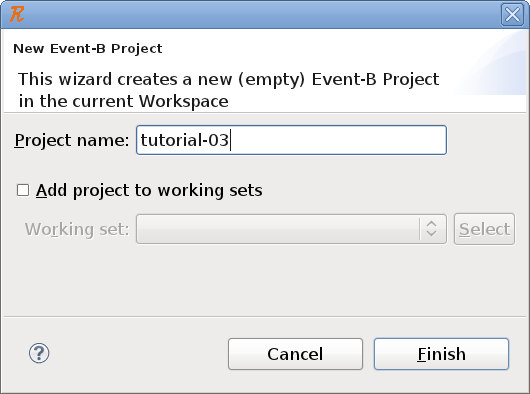
\includegraphics[]{img/tutorial/tut_03_tutorial-3.png}
	\caption{New Event-B Project Wizard}
	\label{fig_tut_03_new_project_wizard}
\end{center}
\end{figure}

\index{project}
\warning{Eclipse supports different types of projects.  The project must have the Rodin Nature (\ref{rodin_nature}) to work.  A project can have more than one nature.}

\index{component}
Next, create a new Event-B Component.  Either use \textsf{File $\rangle$ New $\rangle$ Event-B Component} or right-click on the newly created project and select \textsf{New $\rangle$ Event-B Component}.  Use \texttt{mac} as the component name, select \textsf{Machine} as component-type, and click \textsf{Finish} as shown in Figure \ref{fig_tut_03_new_component_wizard}. This will create a Machine (\ref{machine}) file.

\begin{figure}[!ht]
\begin{center}
	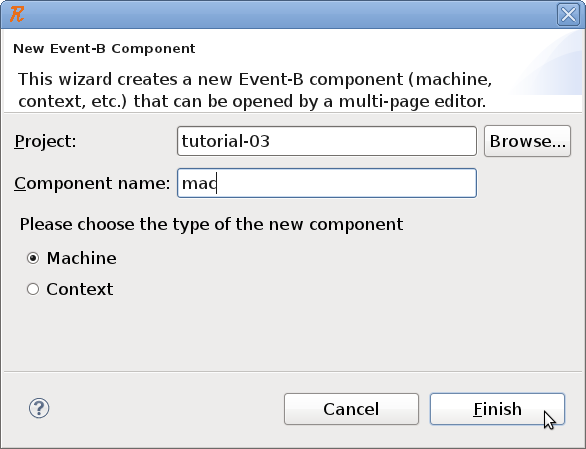
\includegraphics[]{img/tutorial/tut_03_mac.png}
	\caption{New Event-B Component Wizard}
	\label{fig_tut_03_new_component_wizard}
\end{center}
\end{figure}

The newly created component will open in the Rodin Editor. This displays the machine hierarchy as text, although at this point, you cannot add any text apart from comments. Elements can be added to the model by clicking on using the wizards for variables, variants, invariants, and events (the \icon{rodin/newvar_edit.png},\icon{rodin/newvariant_edit.png},\icon{rodin/newinv_edit.png}, and \icon{rodin/newevt_edit.png} buttons). You can also add elements by finding the name of the machine under the MACHINE heading. There is a small green arrow directly to the right of the name of the machine (in this case, the name of the machine is "mac"). Place your cursor directly to the left of the green arrow and right click. Select the element that you would like to add from the \textsf{Add Child} menu. If an element of a certain type has already been created, you can also create more elements of that type right clicking on the type of the element you would like to add (e.g. \textsf{VARIABLES}) that is coloured in purple and select \textsf{Add Child}. You can also place your cursor directly before the green arrow to the left of an element name and hit \textsf{CTRL-T} or right click and select \textsf{Add Sibling}.
\marginpar{Might be good to make a screenshot or at least get a .png of what the little green arrow looks like?}

You can also edit the machine using the Event-B Machine Editor. To do this, right click on the mac component in the Event-B Explorer and select \textsf{Open With $\rangle$ Event-B Machine Editor}. This editor has four tabs at the bottom.  The \textsf{Pretty Print} shows the model as a whole with color highlighting, but it cannot be edited here.  This is useful to inspect the model.  The \textsf{Edit} allows editing of the model.  It shows the six main sections of a machine (REFINES, SEES, etc.) in a collapsed state.  You can click on the \icon{rodin/collapsed.png} button to the left of a section to expand it.

%\begin{figure}[!ht]
%\begin{center}
%	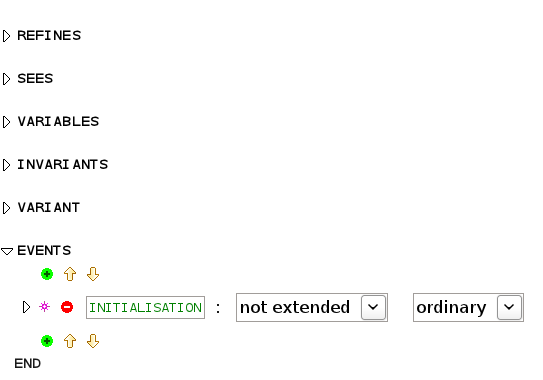
\includegraphics[]{img/tutorial/tut_03_interface.png}
%\end{center}
%\end{figure}

The editor is \textit{form-based}.  This means that in well-defined places an appropriate control (text field, dropdown, etc.) allows modifications. 

\info{Alternative editors are available as plug-ins.  The form editor has the advantage of guiding the user through the model, but it takes up a lot of space and can be slow for big models.  The text-based Camille Editor (\ref{tut_camille}) is very popular.  Please visit the Rodin Wiki (\ref{rodin_wiki}) for the latest information.}

\subsection{Camille, a text-based editor}
\label{tut_camille}
\begin{rodin-plugin}{img/camille.png}{Camille}
Camille is a ``real'' text editor that provides the same feel as a typical Eclipse text editor, including copy and paste, undo, redo, etc.  However, please note that at this time, not all Rodin plugins are compatible with Camille.  Also, please consult the extensive documentation in the Rodin Wiki (\ref{rodin_wiki}).

Camille can be installed via its update site, which is preconfigured in Rodin.  Once installed, Camille is made the default editor.  The structural editor can still be used by selecting it from the context menu of a file in the project browser.

For more information, please visit \url{http://wiki.event-b.org/index.php/Text_Editor}.


\end{rodin-plugin}

\subsection{Building the Model}
\label{tut_building_the_model}

Back to the problem: Our objective is to build a simplified traffic light controller as described in \ref{tut_first_machine}.  We start with the model state.  Two traffic lights will be modelled and we will therefore create two variables called  \texttt{cars\_go} and \texttt{peds\_go}.  

\subsubsection{Creating Variables}
\index{variable!creating a variable}

Under the \textsf{MACHINE} heading, you see the machine name \textsf{mac}. There is a small green arrow to the right of this label. Place your cursor directly to the left of the green arrow, right click, and select \textsf{Add Child $\rangle$ Event-B Variable} to add a new variable. Optionally, you can also use the New Variable Wizard (the button \icon{rodin/newvar_edit.png}) to create your variable. By default, the variable is named \textsf{var1}. Place your cursor inside the \textsf{var1} label. The label turns into a textbox. Change the name to \textsf{cars\_go}. You can add a comment to the variable by placing your cursor to the right of the little green arrow and typing into the text box that appears.

%Go to the \textsf{Edit} tab in the editor and expand the \textsf{VARIABLES} section.  Click on the \icon{rodin/add.png} button to create a new variable.
%You will see two fields. The left one is filled with the word \texttt{var1}.  Change this to \texttt{cars\_go}.  The second field (after the double-slash ``//'') is a comment field in which you can write any necessary notes or explanations.

\index{comment}
\info{\textbf{Comments:} The comment field does not support line breaks, nor is is possible to ``comment out'' parts of the model as it is with most programming languages.}

%\info{\textbf{Comments:} The comment field supports line breaks.  Note that it is not possible to ``comment out'' parts of the model, as is possible with most programming languages.  You can use the comment field to ``park'' predicates and other strings temporarily.}

Create the second variable (\texttt{peds\_go}) in the same way, or place your cursor directly to the left of the small green arrow next to the label \textsf{cars\_go}, and either hit \textsf{CTRL-T} or right click and select \textsf{Add Sibling} from the menu.

%\begin{figure}[!ht]
%\begin{center}
%	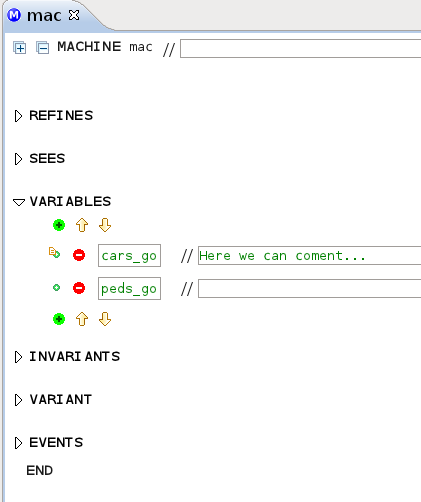
\includegraphics[]{img/tutorial/tut_03_new-variable.png}
%\end{center}
%\end{figure}

Upon saving, the variables will be underlined in red which indicates that an error is present as shown in Figure \ref{fig_tut_03_error}.  The \textsf{Rodin Problems} view (\ref{rodin_problems_view}) shows corresponding error messages. In this case, the error message is ``Variable cars\_go does not have a type''. \marginpar{fig\_tut\_03\_error should be updated to show the new error message}.

\begin{figure}[!ht]
\begin{center}
	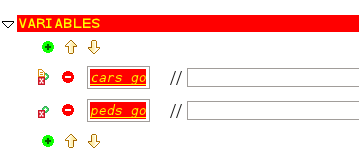
\includegraphics[]{img/tutorial/tut_03_error.png}
	\caption{Red highlighted elements indicate errors}
	\label{fig_tut_03_error}
\end{center}
\end{figure}

Invariants are needed in order to specify the type of variables. Use the method described above to add invariants to your machine (except this time select \textsf{Add Child $\rangle$ Event-B Invariant} from the menu or click the \icon{rodin/newinv_edit.png} button to open up the New Invariant Wizard). Add two invariants (which will automatically be labelled \textsf{inv1} and \textsf{inv2}). The actual invariant appears to the left of the label and is prepopulated with the symbol $\btrue$, which represents the logical value ``true''. Placing your cursor inside the invariant field will change it to a text field and allow editing. 

%Types are provided by invariants. Expand the \textsf{INVARIANTS} section and add two elements by following the same steps as above.  Invariants have labels.  Default labels are generated (\texttt{inv1} and \texttt{inv2}).  The actual invariant is prepopulated with $\btrue$, which represents the logical value ``true''.
Change the first invariant (the $\btrue$, not the label \texttt{inv1}) to $cars\_go \in  BOOL$ and the second invariant to $peds\_go \in  BOOL$.
Event-B provides the build-in datatype \texttt{BOOL} amongst others (\ref{data_types}).

%\begin{figure}[!ht]
%\begin{center}
%	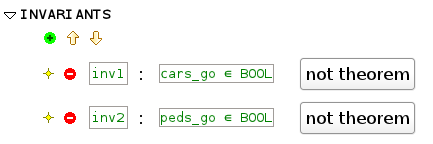
\includegraphics[width=0.7\textwidth]{img/tutorial/tut_03_invariants.png}
%\end{center}
%\end{figure}

\info{\textbf{Mathematical Symbols:} Every mathematical symbol has an ASCII-representation and the substitution occurs automatically.  To generate ``element of'' ($\in$), simply type a colon (``:'').  The editor will perform the substitution after a short delay. The \textsf{Symbols} view shows all supported mathematical symbols. The ASCII representation of a symbol can be found by hovering over the symbol in question.}

\index{yellow highlighting}
After saving, you should see that the \textsf{INITIALISATION} event is underlined in yellow with a small warning sign to the left as demonstrated in Figure~\ref{fig_tut_03_warning}. \marginpar{fig\_tut\_03\_warning needs to be updated} Again, the \textsf{Rodin Problems} view gives us the error message: ``Variable cars\_go is not initialized''. Every variable must be initialized in a way that is consistent with the model.

\begin{figure}[!ht]
\begin{center}
	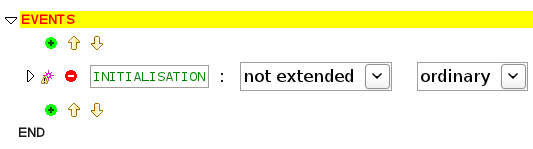
\includegraphics[]{img/tutorial/tut_03_yellow.png}
	\caption{Yellow highlighted elements indicate warnings}
	\label{fig_tut_03_warning}
\end{center}
\end{figure}

To fix this problem, place your cursor to the left of the small green arrow next to the label \textsf{INITIALISATION}. Right click and add an \textsf{Event-B Action}. Repeat to add another event. In the action fields, enter $cars\_go :=  FALSE$ and $peds\_go :=  FALSE$.

%To fix this problem, expand the \textsf{EVENTS} section and then the INITIALIZATION event.  Add two elements in the \textsf{THEN} block.  These are actions that also have labels.  In the action fields, enter $cars\_go :=  FALSE$ and $peds\_go :=  FALSE$.

%\begin{figure}[!ht]
%\begin{center}
%	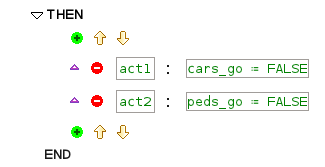
\includegraphics[]{img/tutorial/tut_03_events.png}
%\end{center}
%\end{figure}

\subsubsection{State Transitions with Events}

Our traffic light controller cannot yet change its state.  To make this possible, we create two events (Chapter \ref{events}) in the manner described above and name them \textsf{set\_peds\_go} and \textsf{set\_peds\_stop}. This will model the traffic light for the pedestrians, and for each of these, we will add an Event-B action to each of the events. These actions will change \textsf{peds\_go} to \textsf{TRUE} or \textsf{FALSE}, which simulates the changing of the traffic light.

\warning{From now on, we won't describe the individual steps in the editor any more.  Instead, we will simply show the resulting model.} 

The two events will look as follows:

\pencil{
\begin{description}
	\EVT {set\_peds\_go}
		\begin{description}
		\BeginAct
			\begin{description}
			\nItemX{ act1 }{ peds\_go :=  TRUE }
			\end{description}
		\EndAct
		\end{description}
	\EVT {set\_peds\_stop}
		\begin{description}
		\BeginAct
			\begin{description}
			\nItemX{ act1 }{ peds\_go :=  FALSE }
			\end{description}
		\EndAct
		\end{description}
\end{description}
}

\subsubsection{Event parameters}
\index{parameter}

For the traffic light for the cars, we present a different approach and use only one event with a parameter.  The event will use the new traffic light state as the argument. For this, we need to add an Event-B Event Parameter, which will appear under the heading \textsf{ANY}, and an Event-B Guard, which will appear under the heading \textsf{WHERE}: 

\pencil{
\begin{description}
	\EVT {set\_cars}
		\begin{description}
		\AnyPrm
			\begin{description}
			\ItemX{ new\_value }
			\end{description}
		\WhereGrd
			\begin{description}
			\nItemX{ grd1 }{ new\_value \in  BOOL }
			\end{description}
		\ThenAct
			\begin{description}
			\nItemX{ act1 }{ cars\_go :=  new\_value }
			\end{description}
		\EndAct
		\end{description}
\end{description}
}

Note how the parameter is used in the action block to set the new state.

\subsubsection{Invariants}
\label{tutorial:invariants}
\index{invariant}

If this model was actually in control of a traffic light, we would have a problem because nothing is preventing the model from setting both traffic lights to \texttt{TRUE}.  The reason is that so far we only modeled the domain (the traffic lights and their states) and not the requirements.  We have the following safety requirement:

\begin{center}REQ-1: Both traffic lights must not be \texttt{TRUE} at the same time.\end{center}

We can model this requirement with the following invariant:
\[
\lnot  (cars\_go = TRUE \land  peds\_go = TRUE)
\]
Please add this invariant with the label \texttt{inv3} to the model, use \texttt{not} and \texttt{\&} for $\lnot$ and $\land$.

Obviously, this invariant can be violated, and Rodin informs us of this.  The \textsf{Event-B Explorer} (\ref{eventb_explorer}) provides this information in various ways.  Go to the explorer and expand the project (\texttt{tutorial-03}), the machine (\texttt{mac}) and the entry ``Proof Obligations''.
You should see four proof obligations, two of which are discharged (marked with \icon{rodin/discharged}) and two of which are not discharged (\icon{rodin/pending}).

\index{proof obligation}
\info{\textbf{Proof obligations:} A proof obligation is something that has to be
  proven to show the consistency of the machine, the correctness of theorems, etc.
  A proof obligation consists of a label, a number of hypothesis that can be used
  in the proof and a goal -- a predicate that must be proven.
  Have a look at the proof obligation labels.
  They indicate the origin in the model where they were generated. 
  E.g. \eventbpo{set\_peds\_go/inv3/INV} is the proof obligation that the event  \eventbpo{set\_peds\_go} preserves the invariant (\eventbpo{INV}) with the label \eventbpo{inv3}.
  An overview about all labels can be found in \ref{generated_proof_obligations}.
  The proof obligations can also be found via other entries in the explorer, like the events they belong to.
  Elements that have non-discharged proof obligations as children are marked with a small question mark.  For instance, \texttt{inv3} has all proof obligations as children, while the event \texttt{set\_cars} has one.}

To prevent the invariant from being violated (and therefore to allow all proof obligations to be discharged), we need to strengthen the guards (\ref{guards}) of the events.

\warning{Before looking at the solution, try to fix the model yourself.}

\subsubsection{Finding Invariant Violations with ProB}
\label{tut:prob}
\index{ProB}
\begin{rodin-plugin}{img/prob.png}{ProB}
A useful tool for understanding and debugging a model is a model checker like ProB. You can install ProB from the ProB Update Site, directly from Rodin.  Just select \textsf{Install New Software...} from the \textsf{Help} menu and select ``ProB'' from the dropdown. You should see ``ProB for Rodin2`` as an installation option, which you can then install using the normal Eclipse mechanism.

We will continue the example at the point where we added the safety invariant (REQ-1), but didn't add guards yet to prevent the invariants from being violated.

We launch ProB by right-clicking on the machine we'd like to animate and select \textsf{Start Animation / Model Checking}.  Rodin will switch to the ProB-Perspective, as shown in Figure~\ref{fig_tut_prob_perspective}. The top left pane shows the available events of the machines.  Upon starting, only INITIALIZATION is enabled.  The middle pane shows the current state of the machine, and the right pane shows a history.  On the bottom of the main pane we can see whether any errors occurred, like invariant violations. We can now interact with the model by triggering events.  this is done by double-clicking on an enabled event, or by right-clicking it and selecting a set of parameters, if applicable.  We first trigger INITIALIZATION.  After that, all events are enabled.  Next, we trigger \texttt{set\_cars} and \texttt{set\_peds\_go}  with the parameter $TRUE$.  As expected, we will get an invariant violation.  In the state view, we can ``drill down'' and find out which invariant was violated, and the history view shows us how we reached this state (Figure~\ref{tut_03_prob_invariant_violation}). After modifying a machine, ProB has to be restarted, which is done again by right-clicking the machine and selecting ProB.  Triggering events to find invariant violations is not very efficient.  But ProB can perform model checking automatically.  To do so, select \textsf{Model Checking} from the \textsf{Checks} menu from the ``Events'' View (the view on the left).  After optionally adjusting some parameters, the checking can be triggered by pressing ``Start Consistency Checking".  Upon completion, the result of the check is shown. ProB has many more functions and also supports additional formalisms. Please visit the \href{http://www.stups.uni-duesseldorf.de/ProB}{ProB Website} for more information.

\end{rodin-plugin}

\begin{figure}[!ht]
\begin{center}
	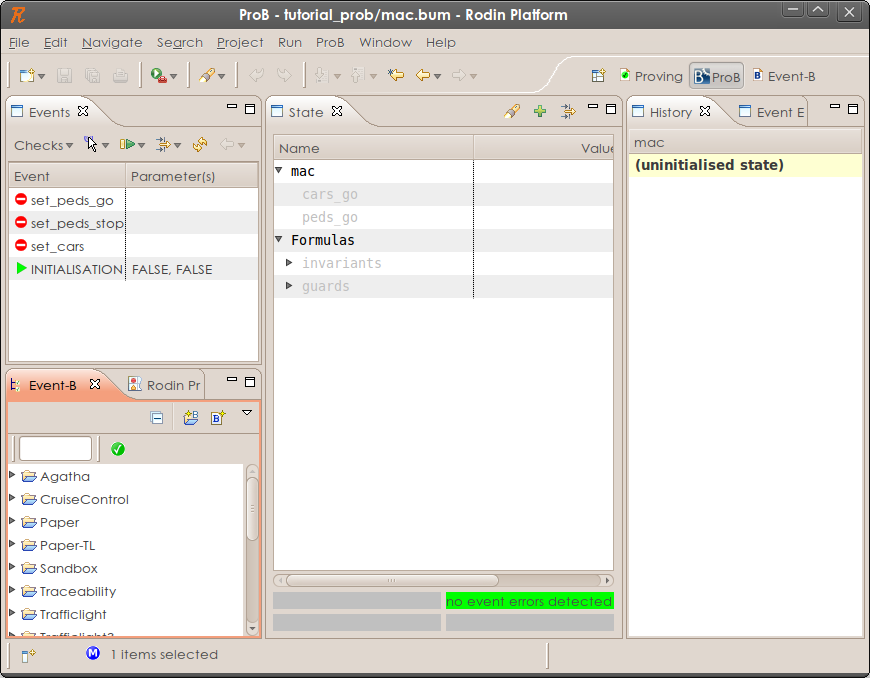
\includegraphics[]{img/tutorial/tut_03_prob_perspective.png}
	\caption{The ProB Perspective}
	\label{fig_tut_prob_perspective}
\end{center}
\end{figure}

\begin{figure}[!ht]
\begin{center}
	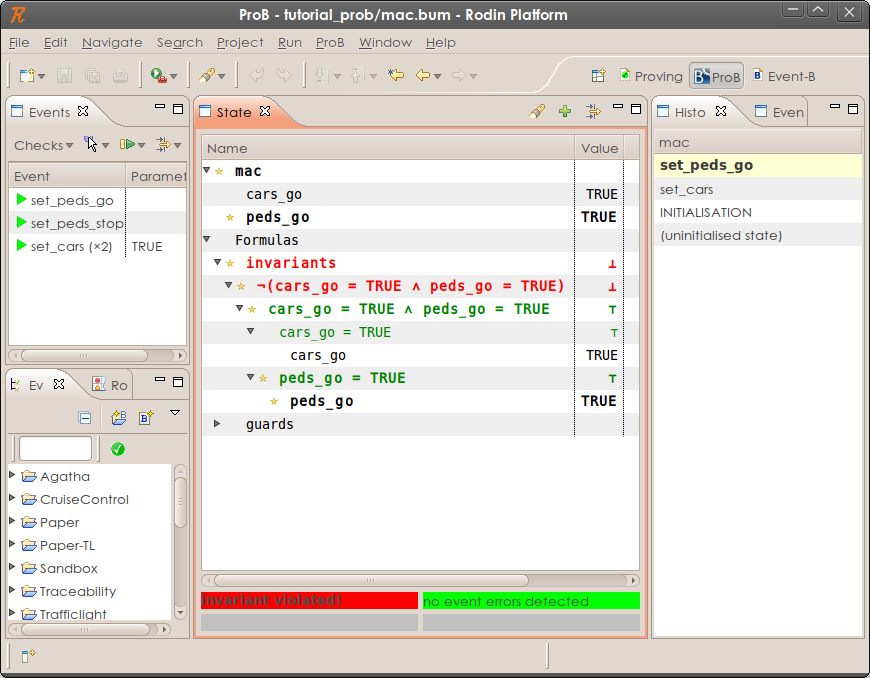
\includegraphics[]{img/tutorial/tut_03_prob_invariant_violation.png}
	\caption{An invariant violation, found by ProB}
	\label{tut_03_prob_invariant_violation}
\end{center}
\end{figure}


\subsection{The Final Traffic Light Model}
\label{tut_final_model}

\pencil{
\begin{description}
\MACHINE{mac}
\VARIABLES
	\begin{description}
		\Item{ cars\_go }
		\Item{ peds\_go }
	\end{description}
\INVARIANTS
	\begin{description}
		\nItemX{ inv1 }{ cars\_go \in  BOOL }
		\nItemX{ inv2 }{ peds\_go \in  BOOL }
		\nItemX{ inv3 }{ \lnot  (cars\_go = TRUE \land  peds\_go = TRUE) }
	\end{description}
\EVENTS
	\INITIALISATION
		\begin{description}
		\BeginAct
			\begin{description}
			\nItemX{ act1 }{ cars\_go :=  FALSE }
			\nItemX{ act2 }{ peds\_go :=  FALSE }
			\end{description}
		\EndAct
		\end{description}
	\EVT {set\_peds\_go}
		\begin{description}
		\WhenGrd
			\begin{description}
			\nItemX{ grd1 }{ cars\_go = FALSE }
			\end{description}
		\ThenAct
			\begin{description}
			\nItemX{ act1 }{ peds\_go :=  TRUE }
			\end{description}
		\EndAct
		\end{description}
	\EVT {set\_peds\_stop}
		\begin{description}
		\BeginAct
			\begin{description}
			\nItemX{ act1 }{ peds\_go :=  FALSE }
			\end{description}
		\EndAct
		\end{description}
	\EVT {set\_cars}
		\begin{description}
		\AnyPrm
			\begin{description}
			\ItemX{ new\_value }
			\end{description}
		\WhereGrd
			\begin{description}
			\nItemX{ grd1 }{ new\_value \in  BOOL }
			\nItemX{ grd2 }{ new\_value = TRUE \limp  peds\_go = FALSE }
			\end{description}
		\ThenAct
			\begin{description}
			\nItemX{ act1 }{ cars\_go :=  new\_value }
			\end{description}
		\EndAct
		\end{description}
\END
\end{description}
}


%%% Local Variables: 
%%% mode: latex
%%% TeX-master: "rodin-doc"
%%% End: 





\chapter{Reference}
\label{reference}

\section{Abstract Machine Notation}
\label{abstract_machine_notation}

\section{Arithmetic}
\label{arithmetic}

\section{Atelier B Provers}
\label{atelier_b_provers}

\section{Camille}
\label{camille}

Camille is an alternative, text-based editor.  It can be installed through the Eclipse Install mechanism.  More information is available in the Rodin Wiki (\ref{rodin_wiki}).

\section{Context}
\label{context}

\section{Data Refinement}
\label{data_refinement}

\section{Datatypes}
\label{datatypes}

List of Event-B datatypes

\section{Eclipse}
\label{eclipse}

- Eclipse Definition

- Pointers to Web Tutorials, etc.

\section{Editor View}
\label{editor_view}


\section{Event}
\label{event}

Definition event

\section{Event-B}
\label{eventb}

Event-B is a formal method (\ref{formal_method}) for system-level modelling and analysis. Key features of Event-B are the use of set theory (\ref{set_theory}) as a modelling notation, the use of refinement (\ref{refinement}) to represent systems at different abstraction levels and the use of mathematical proof to verify consistency between refinement levels.

\paragraph{See Also:}
\begin{itemize}
\item \url{http://www.event-b.org}
\end{itemize}

\section{Event-B Component}
\label{eventb_component}

Machines (\ref{machine}) and Contexts (\ref{context}) are components.

\section{Event-B Explorer}
\label{eventb_explorer}

The View showing the Event-B projects and their content.  In the default Event-B perspective, it is the slim browser on the left edge of the Workspace.  If it is missing, make sure that you use the correct perspective.  You can explicitly enable it with \textsf{Windows $\rangle$ Show View... $\rangle$ Event-B Explorer}.

\section{First Order Predicate Calculus}
\label{first_order_predicate_calculus}


\section{Formal Method}
\label{formal_method}

\section{Gluing Invariant}
\label{gluing_invariant}

\section{Guard}
\label{guard}

\section{IDE}
\label{ide}

Integrated Development Environment

\section{Initialization}
\label{initialization}

Every machine has a special event \texttt{INITIALIZATION} that will be used to initialize the machine's state.

TODO: Determinism, refinement.

\section{Label}
\label{label}

\section{Machine}
\label{machine}

\section{Mathematical Notation}
\label{mathematical_notation}

\section{Menu Bar}
\label{menu_bar}

\section{Naming Convention}
\label{naming_convention}

In this section we describe a recommended naming convention.  Good naming conventions save time -- and nerves.

\section{Outline View}
\label{outline_view}

\section{Partition}
\label{partition}

\section{Proof Obligation}
\label{proof_obligation}

\section{Plugin}
\label{plugin}

\section{Refinement}
\label{refinement}

\begin{description}
	\item[Horizontal Refinement]
	\item[Vertical Refinement]
	\item[Data Refinement]
\end{description}

\paragraph*{See also:}
\begin{itemize}
\item Data refinement in the trafficlight tutorial (\ref{tutorial:data_refinement})
\end{itemize}

\section{Rodin Wiki}
\label{rodin_wiki}

\url{http://wiki.event-b.org/}

\section{Structural Editor}
\label{structural_editor}

\section{Symbols View}
\label{symbols_view}

\section{Predicate Logic}
\label{predicate_logic}

\section{Project}
\label{project}

\section{Proof Obligation Labels}
\label{po_labels}

\section{Propositional Calculus}
\label{propositional_calculus}

\section{Rodin}
\label{rodin}

... Rodin Definition ...


\section{Rodin Platform}
\label{rodin_platform}

\section{Rodin Problems View}
\label{rodin_problems_view}


\section{Rodin Nature}
\label{rodin_nature}

Eclipse Projects can have one or more natures to describe their purpose.  The GUI can then adapt to their nature.  Rodin Projects must have the Rodin-Nature.  If you create an Event-B project, it automatically has the right nature.  If you want to modify an existing project, you can edit the \texttt{.project} file and add the following XML in the \texttt{<natures>} section:

\pencil{
\texttt{<nature>org.rodinp.core.rodinnature</nature>}
}

\section{Sees}
\label{sees}

\section{Set Theory}
\label{set_theory}

... Set Theory Definition ...

\section{Tool Bar}
\label{tool_bar}

\section{Undischarged Proof Obligations}
\label{undischarged_proof_obligations}

\section{Upgrade}
\label{Upgrade}


\section{Witness}
\label{witness}





\chapter{Frequently Asked Questions}
\label{faq}

\section{General Questions}

\subsection{What is Event-B?}
\index{Event-B}

Event-B is a formal method for system-level modelling and analysis. Key features of event-B are the use of set theory as a modelling notation, the use of refinement to represent systems at different abstraction levels and the use of mathematical proof to verify consistency between refinement levels.
More details are available in \url{http://www.event-b.org}.

\subsection{What is the difference between Event-B and the B method?}

Event-B (Section \ref{tut_eventb}) is derived from the \href{http://en.wikipedia.org/wiki/B-Method}{B method}. Both notations have the same \href{http://en.wikipedia.org/wiki/Jean-Raymond_Abrial}{inventor}, and share many common concepts (set-theory, refinement, proof obligations, ...) However, they are used for quite different purposes. The B method is devoted to the development of \textit{correct by construction} software, while the purpose of Event-B is used to model full systems (including hardware, software and environment of operation).

Event-B and the B method use mathematical languages which are similar but do not match exactly (in particular, operator precedences are different).

\subsection{What is Rodin?}
\index{Rodin}

The \textbf{Rodin Platform} is an Eclipse-based IDE for Event-B that provides support for refinement and mathematical proofs. The platform is open source, contributes to the Eclipse framework and can be extended with plugins.

\subsection{Where does the Rodin name come from?}

The Rodin Platform (Section \ref{rodin_platform}) was initially developed within the European Commission funded Rodin project (IST-511599 ), where Rodin is an acronym for ``Rigorous Open Development Environment for Complex Systems”. Rodin is also the name of a famous French sculptor. One of his most famous works is the \href{http://en.wikipedia.org/wiki/The_Thinker}{Thinker}. 

\subsection{Where I can download Rodin?}
\label{faq_where_download_rodin}

Rodin is available for download at the Rodin Download page: \url{http://wiki.event-b.org/index.php/Rodin_Platform_Releases}

\subsection{How to contribute and develop?}

Glad to hear that you want to help!  Please see the \url{http://wiki.event-b.org/index.php/Developer_FAQ} page.

\subsection{My operating system is not supported!  How can I install Rodin on my platform?}
\label{faq_os_not_supported}
At the time of this writing, prebuild versions only a small number of operating systems.  There are two recommended approaches for running Rodin in those situations:
\begin{description}
	\item[Build Rodin from the sources] For users who have some experience in building Java software, they may simply build Rodin from the sources.  For more information, please consult the Developer Documentation in the Rodin Wiki: \url{http://wiki.event-b.org/index.php/Rodin_Developer_Support}
	\item[Run Rodin in a virtual environment] With a fast computer, you can also use a virtual environment (e.g. VirtualBox) and install an operating system into that environment that supports Rodin (e.g. a 32bit version of Linux).
\end{description}

There are other options available for more specialized scenarios (e.g. running 32bit Rodin on a 64bit Linux system).  However, the two approaches outlined above are the least painful ones.

\section{General Tool Usage}

\subsection{Do I lose my proofs when I clean a project?}
\index{project!clean}
No! This is a common misunderstanding of what a project clean does. A project contains two kinds of files: 

\begin{itemize}
	\item those you can edit: contexts, machines, proofs 
	\item those generated by a project build: proof obligations, proof statuses (for each proof obligation, discharged or not discharged) 
\end{itemize}

The cleaner just undoes what the builder does, i.e. it removes proof obligations and statuses, but it never modifies any proof.

A status may change from \emph{discharged} to \emph{not discharged} when the proof is no longer compatible with the corresponding proof obligation (e.g. when a hypothesis is changed), but \textbf{the proof itself is still there!}
You can try to \href{http://wiki.event-b.org/index.php/Proof_Obligation_Commands#Proof_Replay_on_Undischarged_POs}{replay} it.

Confusion may arise when automatic provers have been launched. The cleaner does not undo these automatic proofs (why would it ?!!). Once a proof is made, the platform does not modify or delete it by itself. Even \href{http://wiki.event-b.org/index.php/Proof_Purger_Interface#Why_proofs_become_obsolete}{obsolete} proofs are preserved!

\subsection{How do I install external plug-ins without using Eclipse Update Manager?}

Although it is recommended that you install additional plug-ins into the Rodin platform using the Update Manager of Eclipse, this might not always be practical. In this case, you can install these plug-ins by emulating the operations normally performed by the Update Manager either manually or by using ad-hoc scripts. 

The manual installation of plug-ins is described in \href{http://wiki.event-b.org/index.php/Installing_external_plug-ins_manually}{\emph{Installing external plug-ins manually}}. 

\subsection{The builder takes too long}

Generally, the builder spends most of its time attempting to prove POs. There are basically two ways to get it out of the way: 

\begin{itemize}
	\item the first one is to disable the automated prover in the \textsf{Preferences} panel. 
	\item the second one is to mark a PO as reviewed if you do not want the auto-prover to attempt it anymore. 
\end{itemize}

Note that if you disable the automated prover, you always can run it later on some files by using the contextual menu in the Event-B Explorer. 

To disable the automated prover, open \textsf{Rodin Preferences} 
(menu \textsf{Window $\rangle$ Preferences...}). In the tree on the left-hand panel, select \textsf{Event-B $\rangle$ Sequent Prover $\rangle$ Auto-tactic}. Then, in the right-hand panel ensure that the checkbox labelled \textsf{Enable auto-tactic} for proving is disabled. 

To review a proof obligation, just open it in the interactive prover and then click on the \emph{review} button (this is a round blue button with a \emph{R} in the proof control toolbar). The proof obligation should now labelled with the same icon in the Event-B explorer. 

\subsection{What are the ASCII shortcuts for mathematical operators}
\index{symbols}

The ASCII shortcuts that can be used for entering mathematical operators are described in the following section: \textsf{Rodin Keyboard User Guide $\rangle$ Getting Started $\rangle$ Special Combos}. 

This page is also available in the dynamic help system. The advantage of using dynamic help is that it is able to display the help page side-by-side with the other views and editors. To start the dynamic help, click \textsf{Help $\rangle$ Dynamic Help}, then click \textsf{All Topics} and select the page in the tree. 

\subsection{Rodin (and Eclipse) doesn't take into account the MOZILLA\_FIVE\_HOME environment variable}

You have to add a property by appending the following code to your \textsf{eclipse/eclipse.ini} or \textsf{rodin/rodin.ini} file: 

\begin{verbatim} 
	-Dorg.eclipse.swt.browser.XULRunnerPath=/usr/lib/xulrunner/xulrunner-xxx 
\end{verbatim} 

\subsection{No More Handles}

On Windows platforms, it may happen that Rodin crashes, complaining that there are ``no more handles''. This is an OS specific limitation, described \href{http://journals.jevon.org/users/jevon-phd/entry/19833}{here} and \href{https://bugs.eclipse.org/bugs/show_bug.cgi?id=211124}{there}. A workaround is provided at \href{http://blogs.msdn.com/b/ntdebugging/archive/2007/01/04/desktop-heap-overview.aspx}{this site}. 

\subsection{Software installation fails}

The installation of software from update sites (\textsf{Help $\rangle$ Install New Software...}) sometimes fails with an error saying something like: 

\begin{verbatim}
No repository found containing: osgi.bundle,org.eclipse.emf.compare,1.0.1.v200909161031
No repository found containing: osgi.bundle,org.eclipse.emf.compare.diff,1.0.1.v200909161031
...
\end{verbatim}

This is an eclipse/p2 bug, referenced \href{http://stackoverflow.com/questions/511367/error-when-updating-eclipse}{here}. 

The workaround is to: 

\begin{itemize}
	\item Go to \textsf{Window $\rangle$ Preferences $\rangle$ Install/Update $\rangle$ Available Software Sites} 
	\item Remove all sites then add them back again, which can be achieved in the \textsf{Available Software Sites} preference page by: 
	\item Select all update sites (by highlighting them all those that are checked) 
	\item Export them 
	\item Remove them
	\item Restart Rodin
	\item Go back to the preference page and import update sites back (from the previously exported file) 
\end{itemize}

\section{Modeling}
\index{modeling}

\subsection{Witness for \textsf{Xyz} missing. Default witness generated}

A parameter has disappeared during a refinement. If this is intentional, you have to add a witness \ref{witness} telling how the abstract parameter is refined. 

\subsection{Identifier \textsf{Xyz} should not occur free in a witness}

You refer to \textsf{Xyz} in a witness predicate where \textsf{Xyz} is a disappearing abstract variable or parameter which is not set as the witness label. 

\subsection{In \textsf{INITIALISATION}, I get Witness \textsf{Xyz} must be a disappearing abstract variable or parameter}
\index{witness}

The witness is for the after value of the abstract variable, hence you should use the primed variable. The witness label should be \textsf{Xyz'}, and the predicate should refer to \textsf{Xyz'} too. 

\subsection{I've added a witness for \textsf{Xyz} but it keeps saying ``Identifier \textsf{Xyz} has not been defined''}

As specified in the \ref{witness} section, the witness must be labelled by the name \textsf{Xyz} of the concrete variable being concerned.

\subsection{How can I create a new Event-B Project?}
\index{project}

Please check Tutorial \ref{tut_project_setup} to learn how to create a new Event-B project.

\subsection{How to remove a Event-B Project?}

In order to remove a project, first select it on the \textsf{Project Explorer} and then right click with the mouse. The contextual menu will appear on the screen as indicated in Figure \ref{fig_faq_removeproject}.

\begin{figure}[!ht]
\begin{center}
	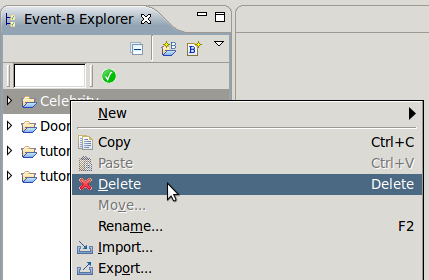
\includegraphics{img/faq/faq_removeproject.png}
	\caption{Removing a Event-B Project}
	\label{fig_faq_removeproject}
\end{center}
\end{figure}

You simply click on \textsf{Delete} and your project will be deleted (after you confirm it in the window that pops up). It is then removed from the \textsf{Project Explorer}.

\subsection{How to export an Event-B Project?}

Exporting a project is the operation by which you can construct automatically a ``zip" file containing the entire project. Such a file is ready to be sent by mail. Once received, an exported project can be imported (next section). It then becomes a project like the other ones which were created locally. In order to export a project, first select it, and then click on \textsf{File $\rangle$ Export...} from the menubar as indicated in Figure \ref{fig_faq_exportproject}. 

\begin{figure}[!ht]
\begin{center}
	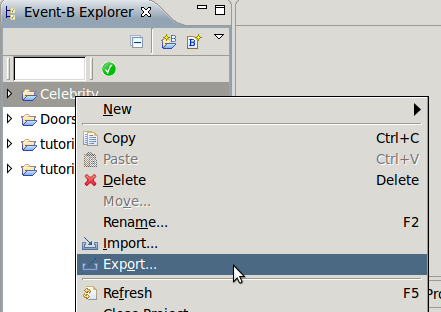
\includegraphics{img/faq/faq_exportproject.png}
	\caption{Export a Event-B Project}
	\label{fig_faq_exportproject}
\end{center}
\end{figure}

The Export wizard will pop up. In this window, select \textsf{General $\rangle$ Archive File} and click the \textsf{Next $>$} button. Specify the path and name of the archive file into which you want to export your project and finally click \textsf{Finish}. This menu sequence belongs to Eclipse (as well as the various options). For more information, refer to the Eclipse documentation. 

\subsection{How to import a Event-B Project?}

A ``.zip" file corresponding to a project which has been exported elsewhere can be imported locally. In order to do this, click on \textsf{File $\rangle$ Import} from the menubar. In the import wizard, select \textsf{General $\rangle$ Existing Projects into Workspace} and click \textsf{Next $>$}. Then, enter the file name of the imported project and finally click \textsf{Finish}. As with exporting, the menu sequence and layout are part of Eclipse.

The importation will fail if the name of the imported project (not the name of the file) is the same as the name of an existing local project. The moral of the story is that when exporting a project to a partner you need to modify its name in case your partner already has a project with that same name (which could be a previous version of the exported project). Changing the name of a project is explained in the next section. 

\subsection{How to change the name of a Event-B Project?}

Select the project whose name you want to modify, and then click on \textsf{File $\rangle$ Rename...}. Modify the name and click on \textsf{OK}. The name of your project will then have been modified accordingly. 

\subsection{How to create a Event-B Component}

Please check Tutorial \ref{tut_project_setup} to learn how to create a new Event-B component.

\subsection{How to remove a Event-B Component}

In order to remove a component, press the right mouse button on the component. In the context menu, select \textsf{Delete}. This component is removed from the \textsf{Project Explorer}. 

\subsection{In the new Rodin Editor, how can I add an element to machine?}
\label{faq_new_editor_new_element}

\info{Please also consult section~\label{new_eventb_editor}, which describes the editor.}

Whenever using the context menu of the new editor, please pay attention to the following two issues:
\begin{itemize}
	\item Make sure that the cursor already is on the correct line.  If you right-click and the cursor is on the wrong line, you will get an incorrect context menu.
	\item Make sure the cursor is not in ``edit'' mode, where you can edit a textual element.  In that scenario you will also get an incorrect context menu.
\end{itemize}

The different elements of the machine, can of course, be added using the different wizards for element creation (New Variable Wizard \icon{rodin/newvar_edit.png}, New Variant Wizard \icon{rodin/newvariant_edit.png}, New Invariant Wizard \icon{rodin/newinv_edit.png}, and New Event Wizard \icon{rodin/newevt_edit.png}) which are described in more detail in Chapter \ref{eventb_editor}. 

You can also add new elements by placing your cursor directly to the left of the small green arrow that appears next to your machine name in \textsf{MACHINE} section. Now right click and select the component that you want to add from the \textsf{Add Child} menu. You can also add an element by right clicking on the heading of the section of the element you want to add (e.g. \textsf{VARIABLES}) and selecting \textsf{Add Child}, or by placing your directly to the left of the small green arrow next to the name of any of the components that already exist and selecting \textsf{Add Sibling}. Unfortunately, the if your cursor is not directly next to the small green arrow (while the cursor is blinking, the left side of the arrow is actually touching the cursor), these methods do not actually work. 

\subsection{How can I use multiple lines for a comment, predicate or expression (using the new editor)?}

To insert a linebreak while editing any field, use Ctrl-Return.

\subsection{How to save a Context or a Machine}

Once a machine or context is (partially) edited, you can save it by using the save button as indicated in Figure \ref{fig_faq_saveaction}.

\begin{figure}[!ht]
\begin{center}
	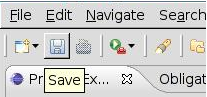
\includegraphics{img/faq/faq_saveaction.png}
	\caption{Save a context or a machine}
	\label{fig_faq_saveaction}
\end{center}
\end{figure}

Once a ``Save" is done, three tools are called automatically, these are:

\begin{itemize}
	\item the Static Checker
	\item the Proof Obligation Generator (Section \ref{generated_proof_obligations})
	\item the Auto-Prover (Section \ref{auto_prover})
\end{itemize}

This can some time. A ``Progress" window can be opened at the bottom right of the screen to see which tools are working (most of the time, it will be the auto-prover). 

\section{Proving}
\index{proving}

\subsection{Help!  Proving is difficult!}

Yes, it is.  Check out Section~\ref{use_provers_effectively} to get started with using the provers.

\subsection{How can I do a Proof by Induction?}

\href{http://wiki.event-b.org/index.php/Induction_proof}{This page about proof by induction} will give you some starting tips.

\subsection{Labels of proof tree nodes explained}

\begin{itemize}
	\item \textsf{ah} means \textit{add hypothesis},
	\item \textsf{eh} means rewrite with \textit{equality from hypothesis} from left to right,
	\item \textsf{he} means rewrite with \textit{equality from hypothesis} from right to left,
	\item \textsf{rv} tells us that this goal has been manually reviewed (see \ref{proof_control_view}),
	\item \textsf{sl/ds} means \textit{selection/deselection},
	\item \textsf{PP} means \textit{discharged by the predicate prover},
	\item \textsf{ML} means \textit{discharged by the mono lemma prover}
\end{itemize}

\section{Usage Questions}

\subsection{Where did the GUI window go?}

When you are looking for a particular view, and the view does not appear or if it appears in a different place than is usual, try clicking on \textsf{Window $\rangle $ Reset Perspective...}. This will reset the different views back to their default positions. If you can't find menu buttons from one of the views, try resizing the view in question to see if part of the menu has been hidden.

\subsection{Where vs. When: What's going on?}
\index{when}
\index{where}

You may have noticed that both in this tutorial, as well as in the tool, events sometimes use the keyword ``when'' and sometimes ``where''.  The idea of this was to make the formal statements more intuitive.  Unfortunately, this created more confusion than anything else.

The short answer is: ``when'' and ``where'' in events have exactly the same meaning, for all practical purposes.

The long answer is: In some contexts (but not all), the tool changes the keywords to make the meaning of the event more apparent.  The distinguishing factor is the parameter: Without parameter, ``when'' is used, with a parameter, ``where'' is used.

To confuse things even more, this doesn't apply everywhere: The structural editor always shows ``where'', but the pretty print toggles between the two.  The Event-B in this handbook has been generated with the \LaTeX plugin, which also toggles the keyword.

%%% Local Variables: 
%%% mode: latex
%%% TeX-master: "rodin-doc"
%%% End: 


\clearpage
\phantomsection
\addcontentsline{toc}{chapter}{Index} 
\printindex

\end{document}

